% \begin{wrapfigure}[15]{R}{0.4\textwidth}
% 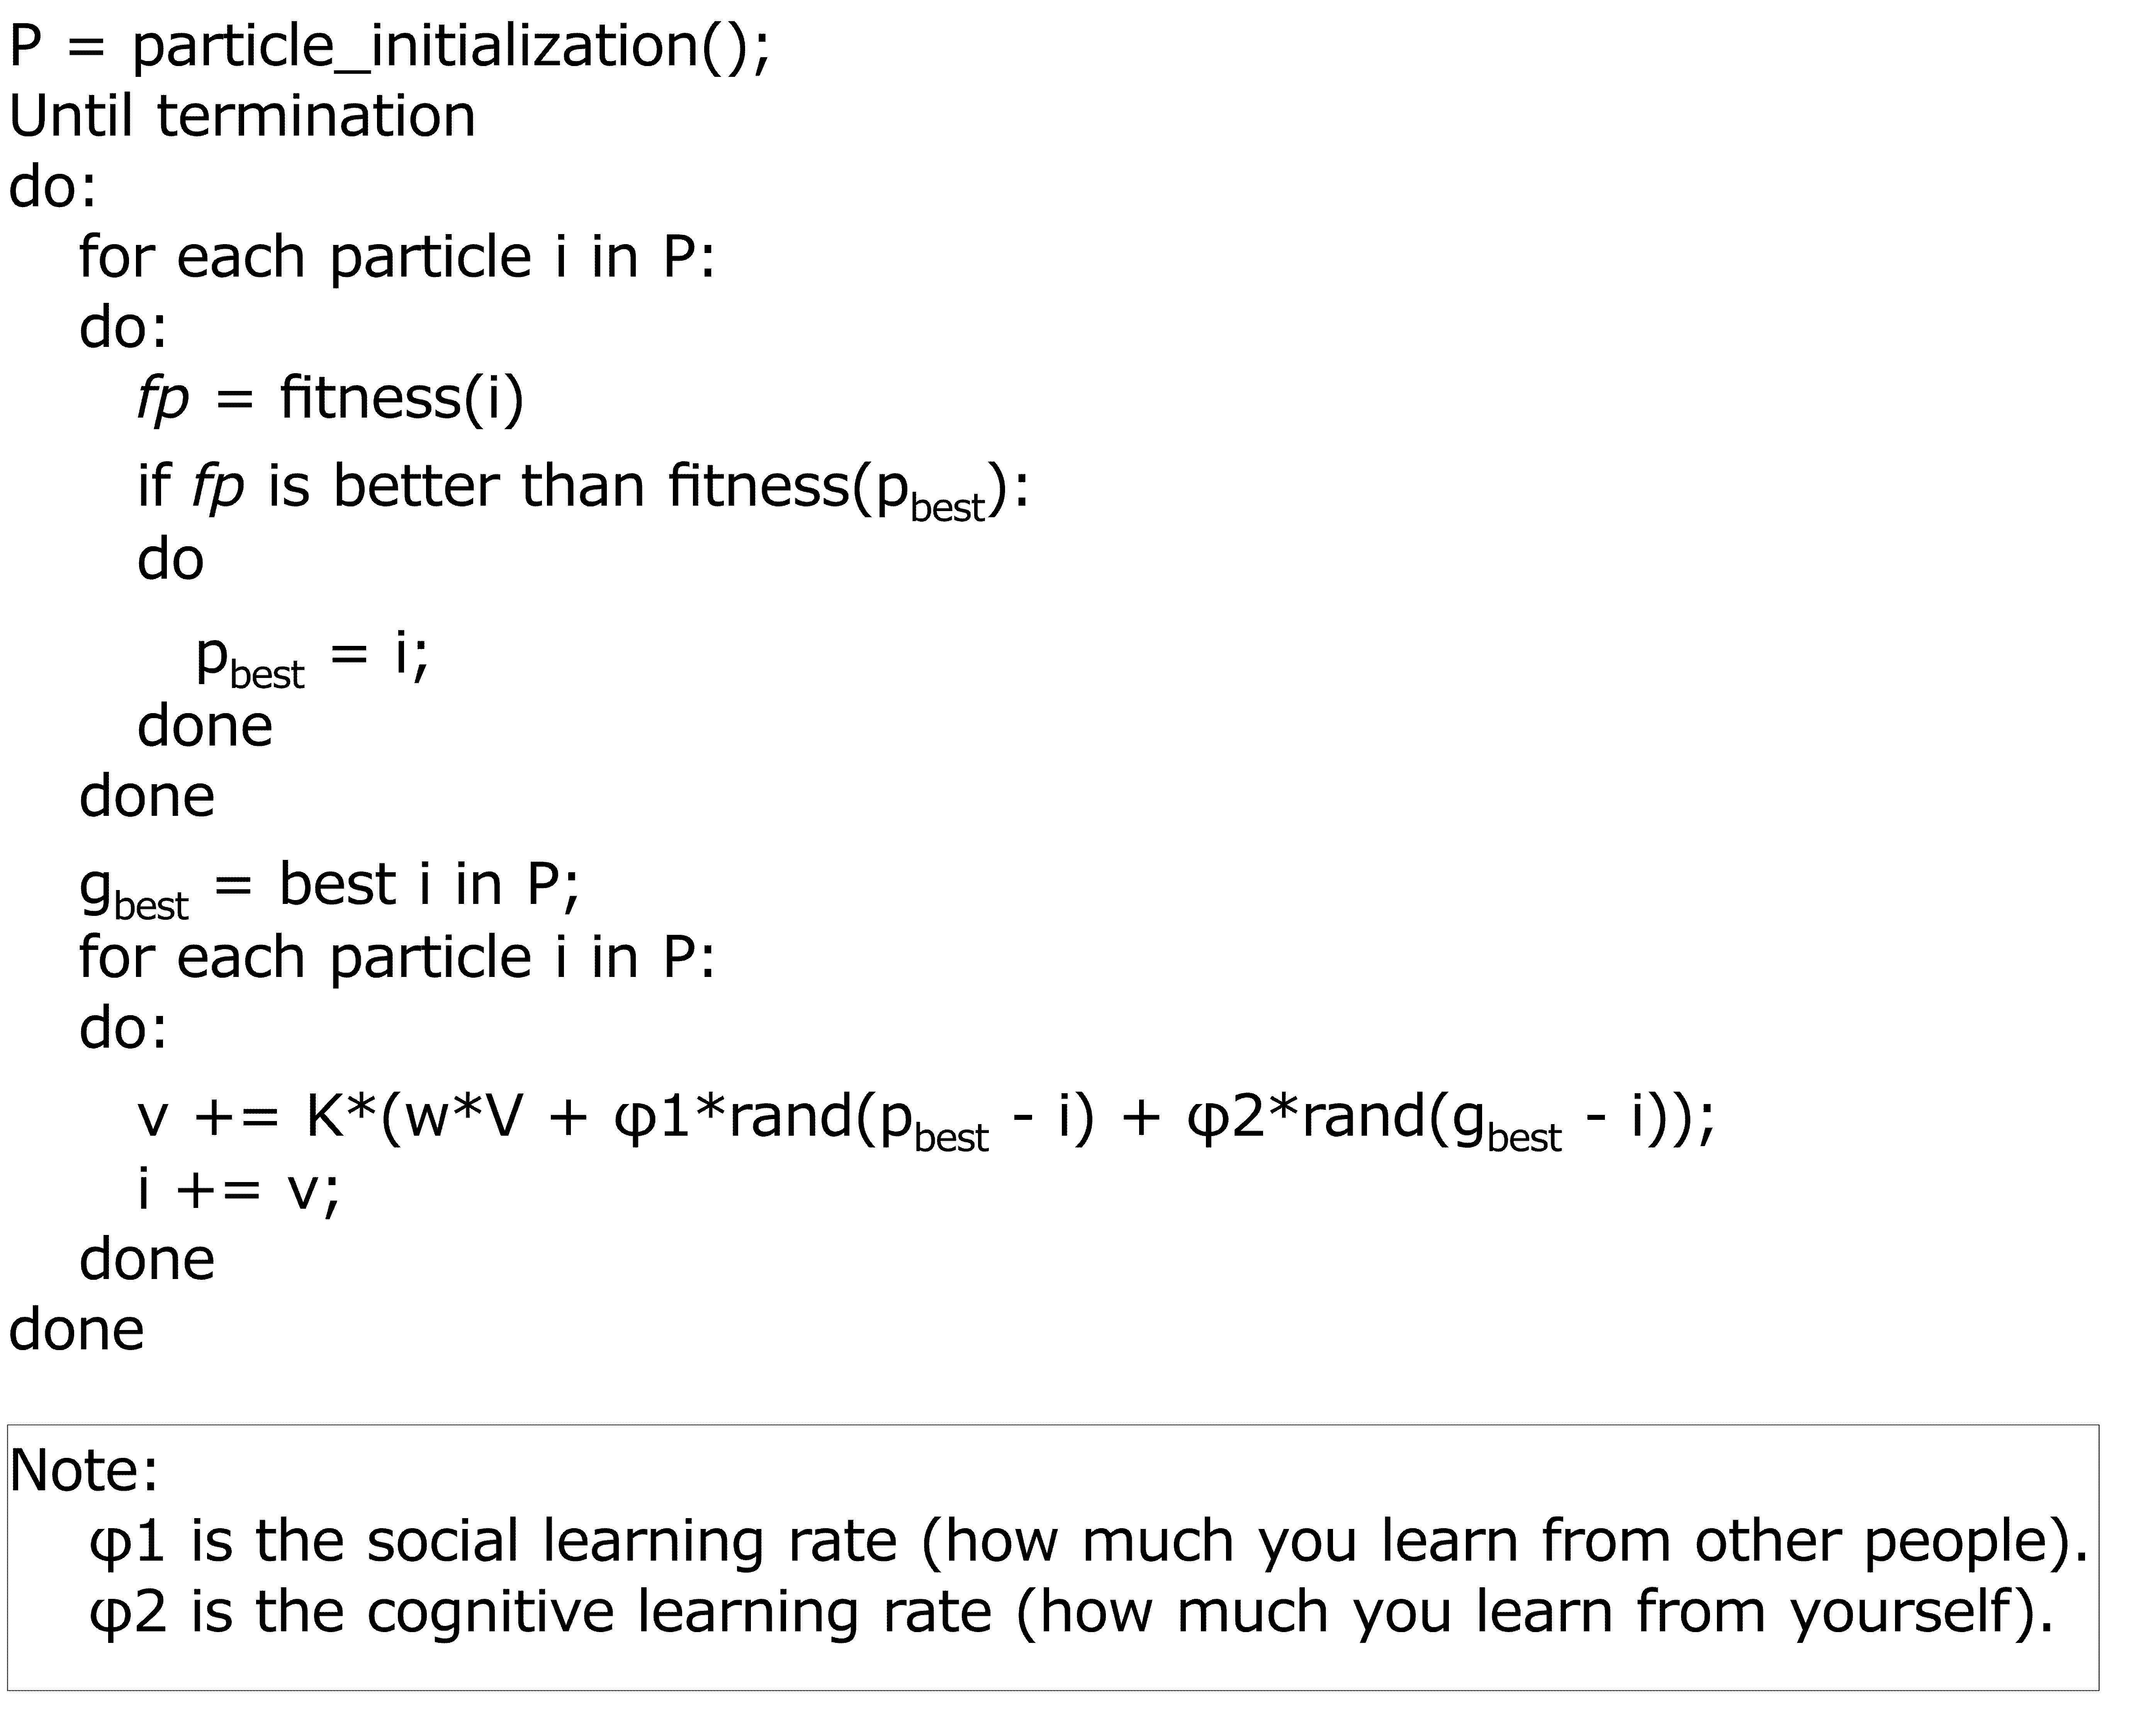
\includegraphics[width=\linewidth]{figs/pso_pseudo.png}
% \caption{Pseudocode for a basic PSO.}
% \label{fig:pso_pseudo}
% \end{wrapfigure}

\begin{figure}[!b]
\begin{minipage}{0.5\linewidth}
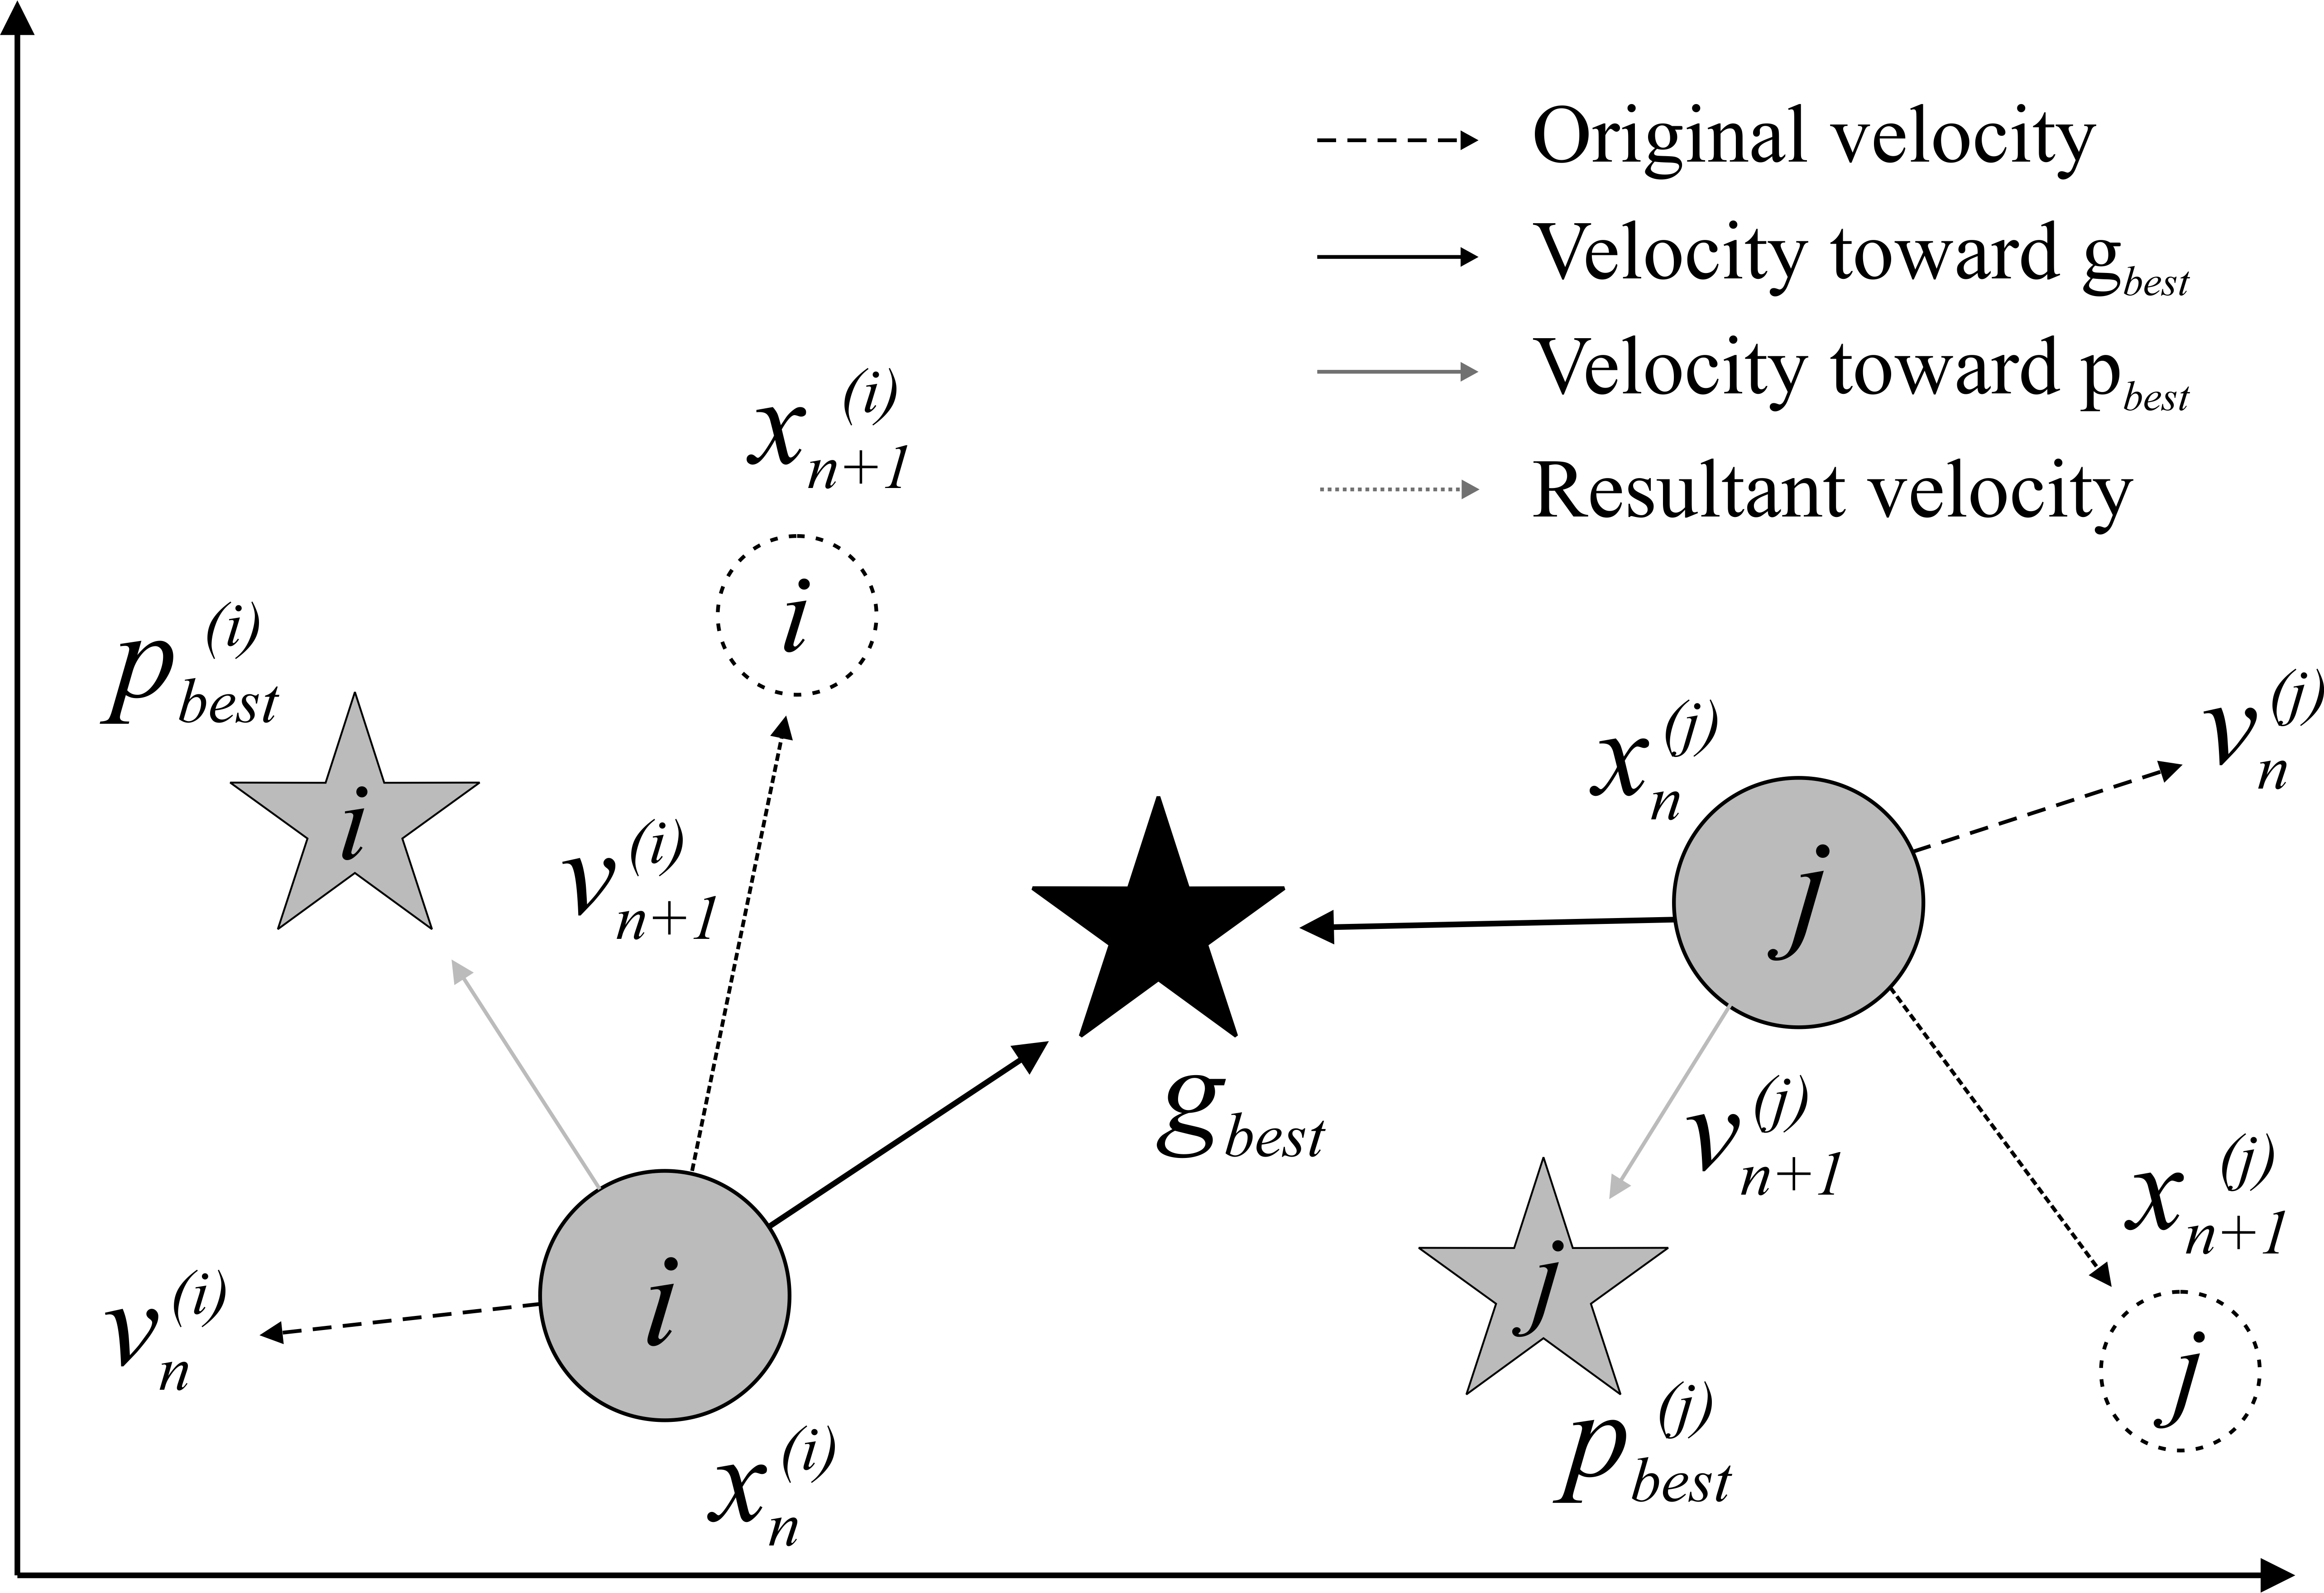
\includegraphics[width=\linewidth]{figs/pso_demo.png}
\caption{Mutations in PSO.}
\label{fig:pso}
\end{minipage}~~~~\begin{minipage}{0.5\linewidth}
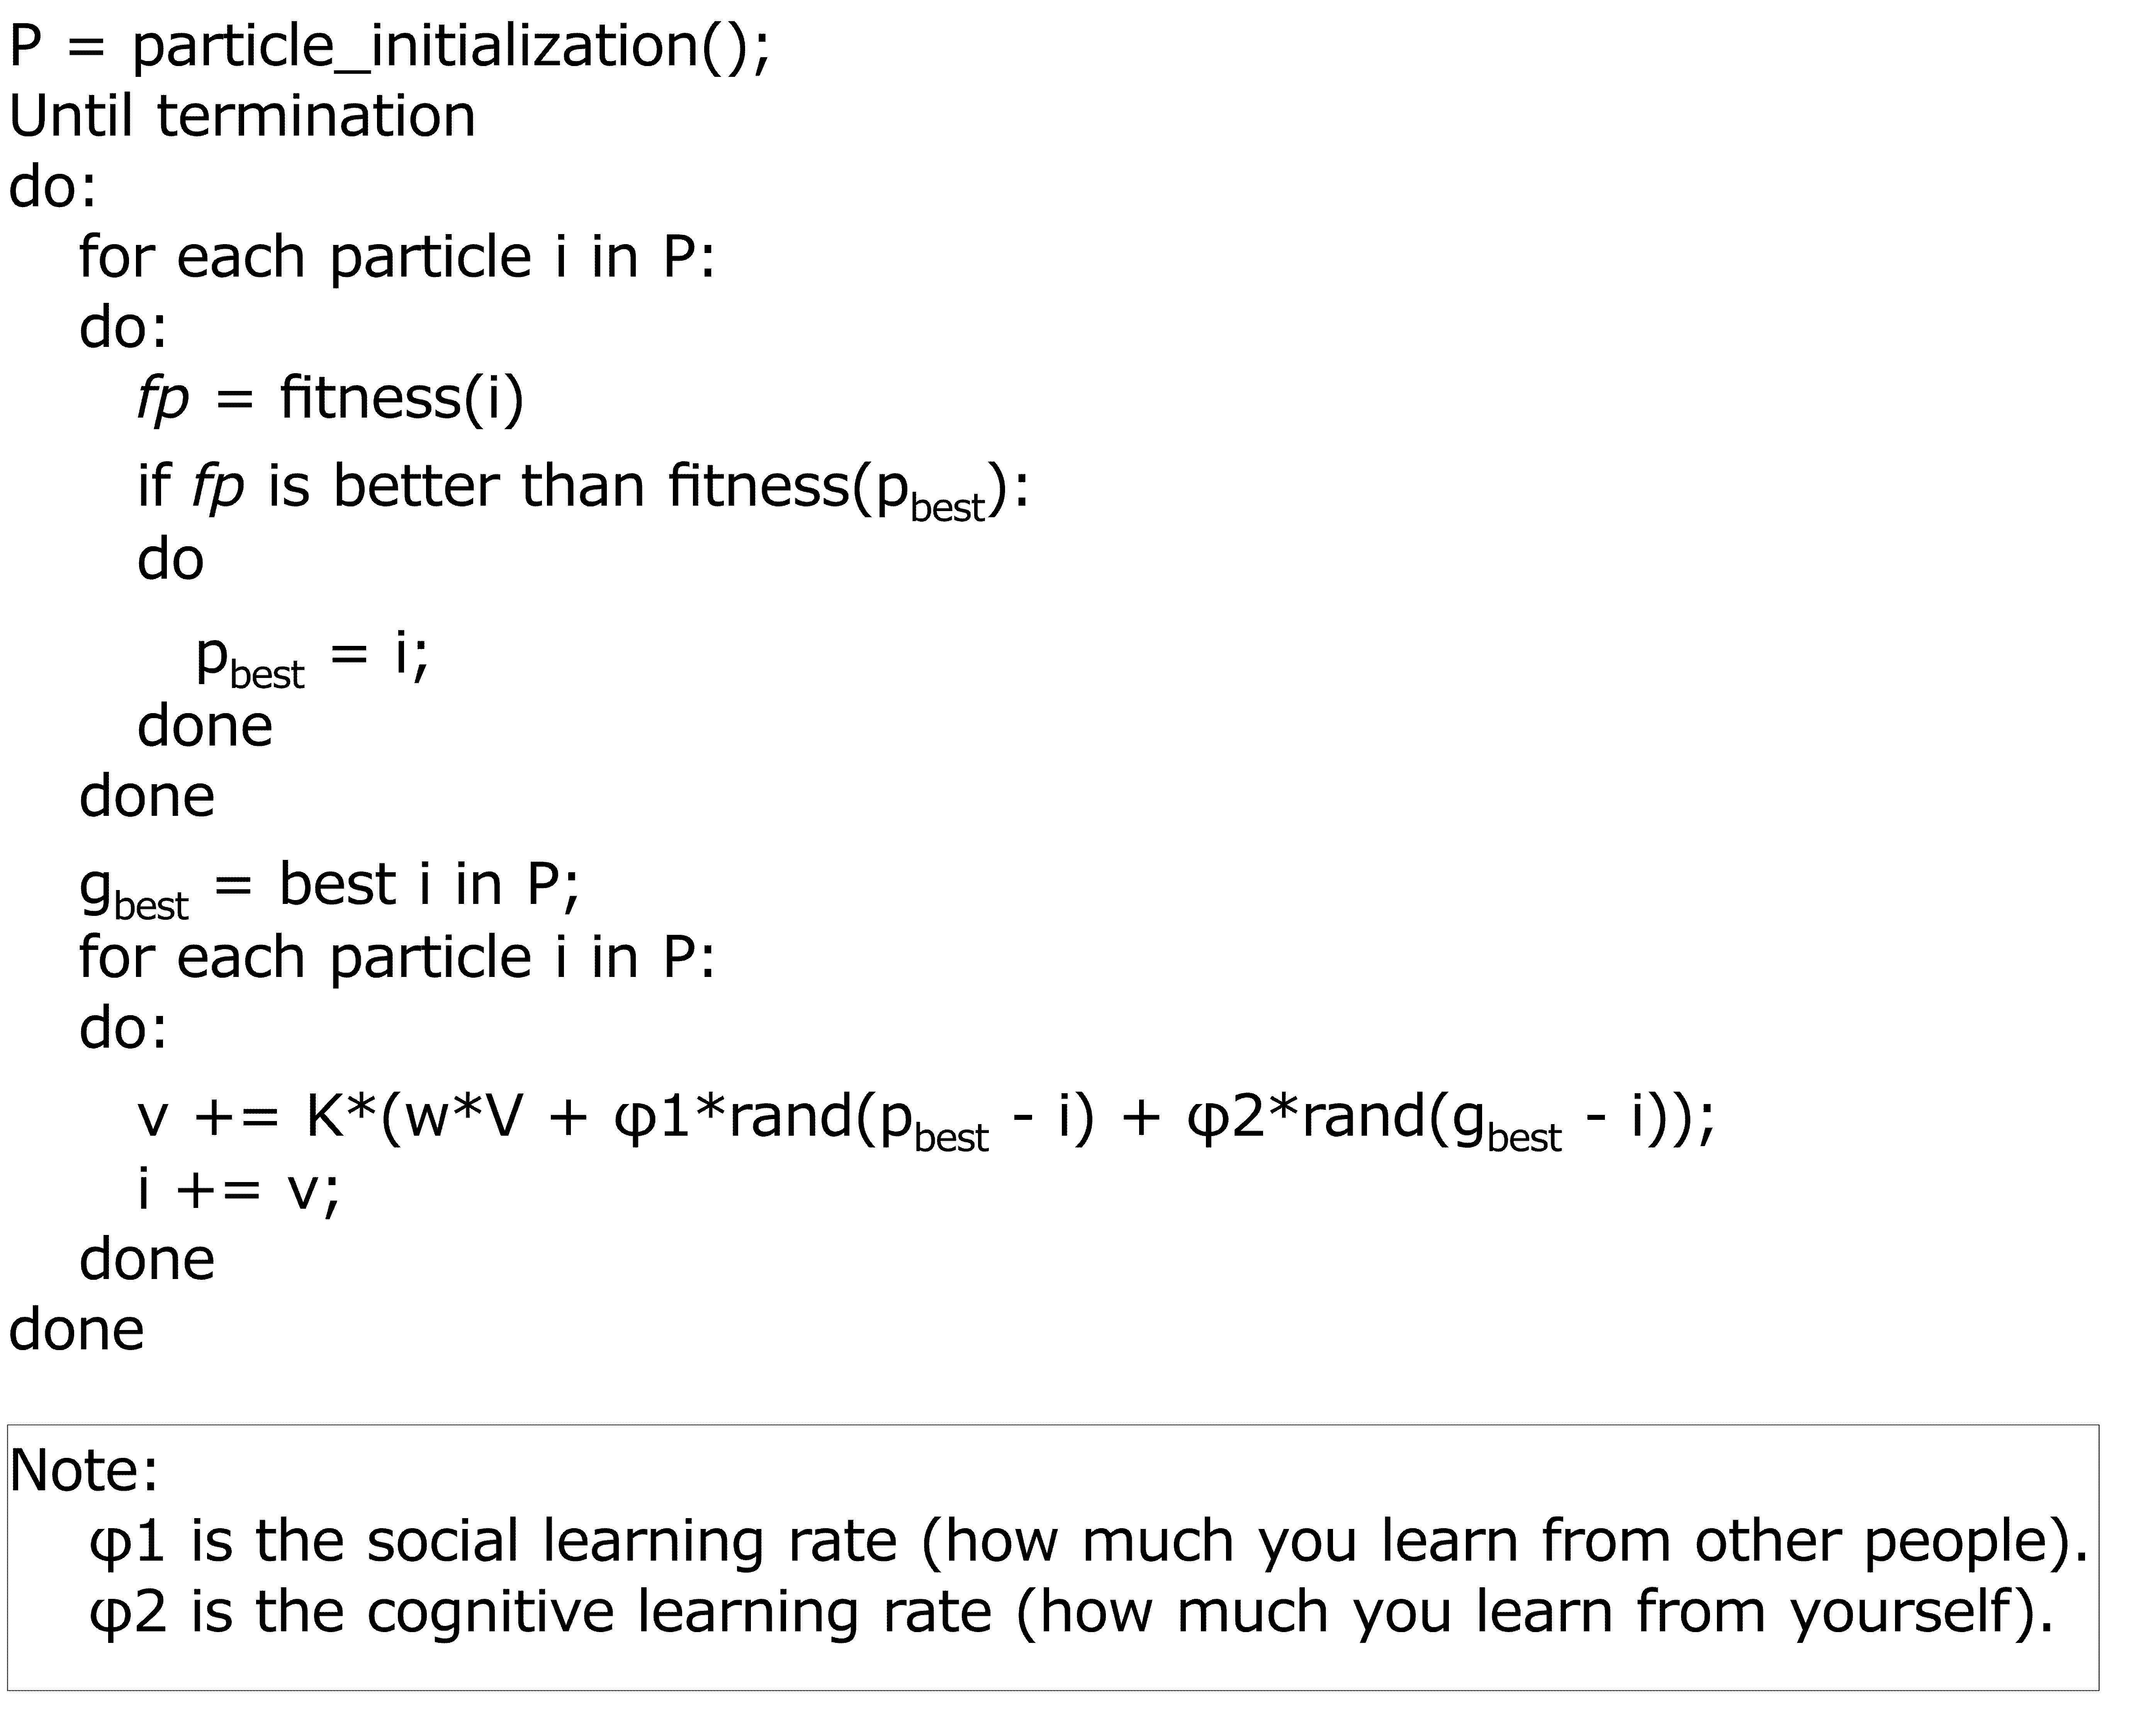
\includegraphics[width=\linewidth]{figs/pso_pseudo.png}
\caption{Pseudocode for a basic PSO.}
\label{fig:pso_pseudo}
\end{minipage}
\end{figure}

% \begin{wrapfigure}[15]{R}{0.4\textwidth}
% 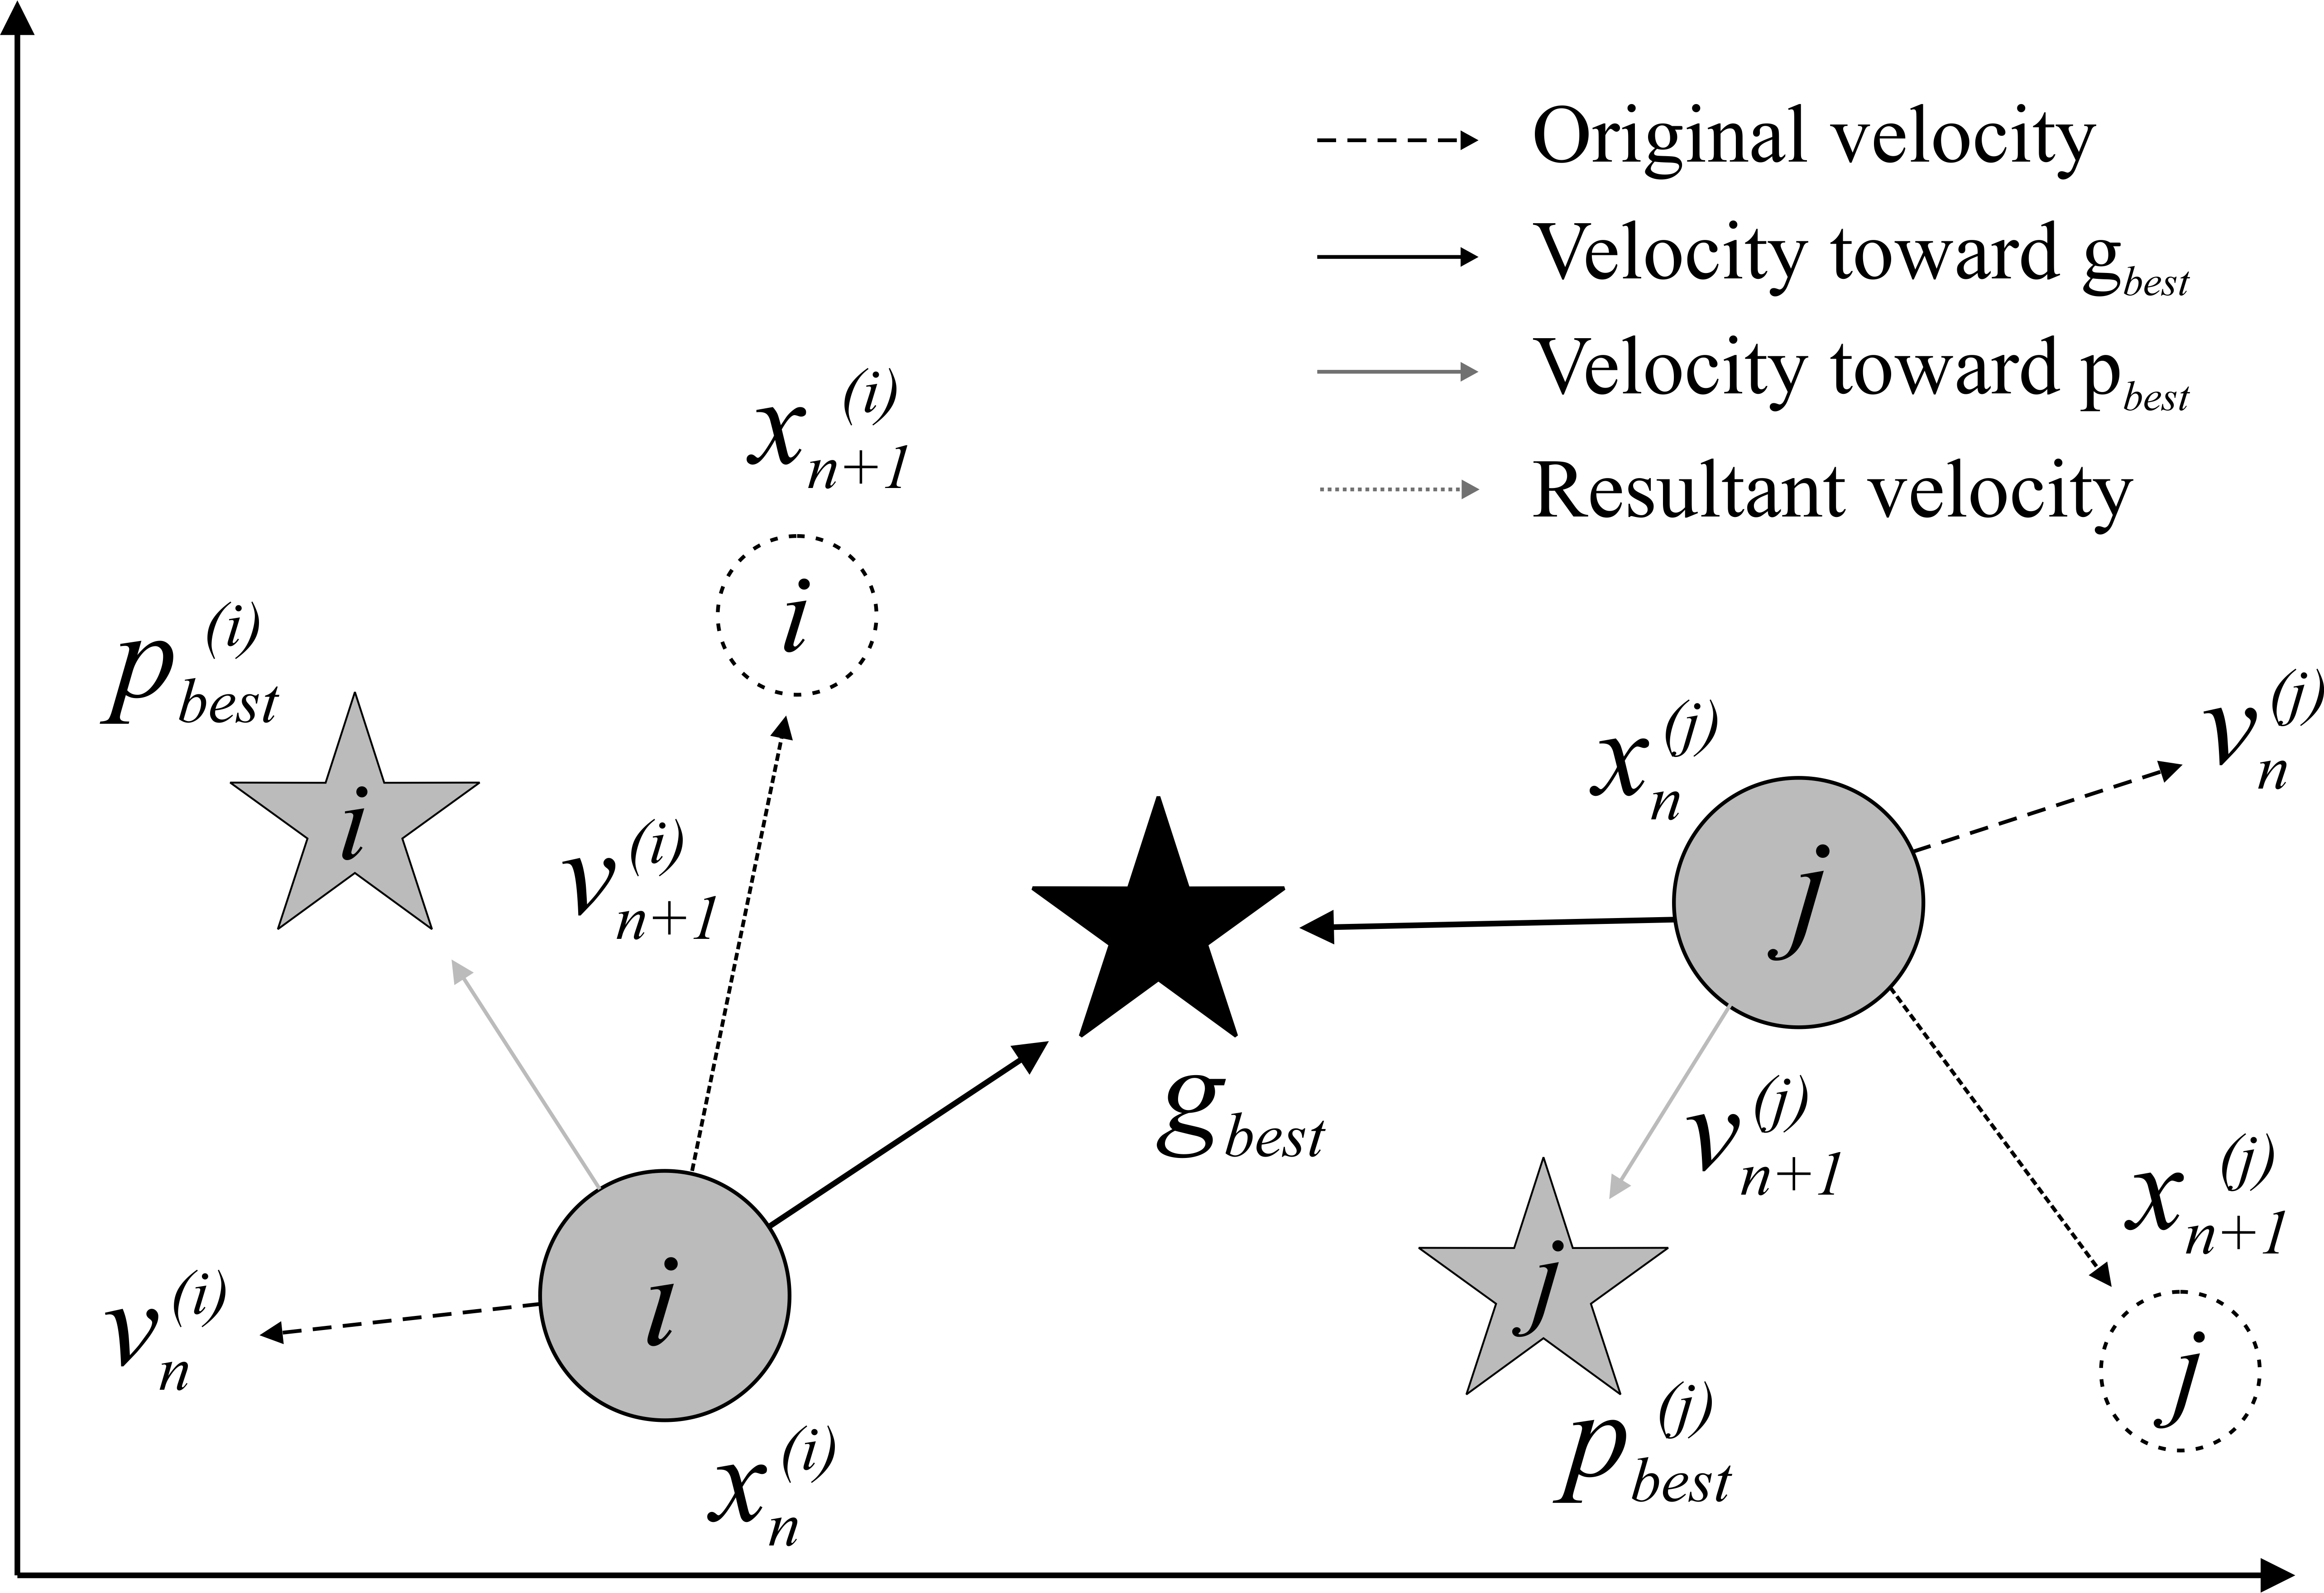
\includegraphics[width=\linewidth]{figs/pso_demo.png}
% \caption{PSO uses sociocognition to mutate its particles. Each particle $i$  mutates in the direction
% $v_n^{(i)}$ while also pulled towards
% (1)~the best idea it ever saw in the past $p_{\mathit{best}}^{(i)}$
% as well as (2)~the best idea ever seen by the community 
% $g_{\mathit{best}}$. As a result, the particle $i$ is redirected towards $x_{n+1}^{i}$.}
% \label{fig:pso}
% \end{wrapfigure}

